\chapter{Results} \label{sec:results}

\section{Linear Behaviour}
Validate with "small analytical model" Domenico suggested in his email.

% figure of the model
\begin{figure}[ht!]
    \centering
    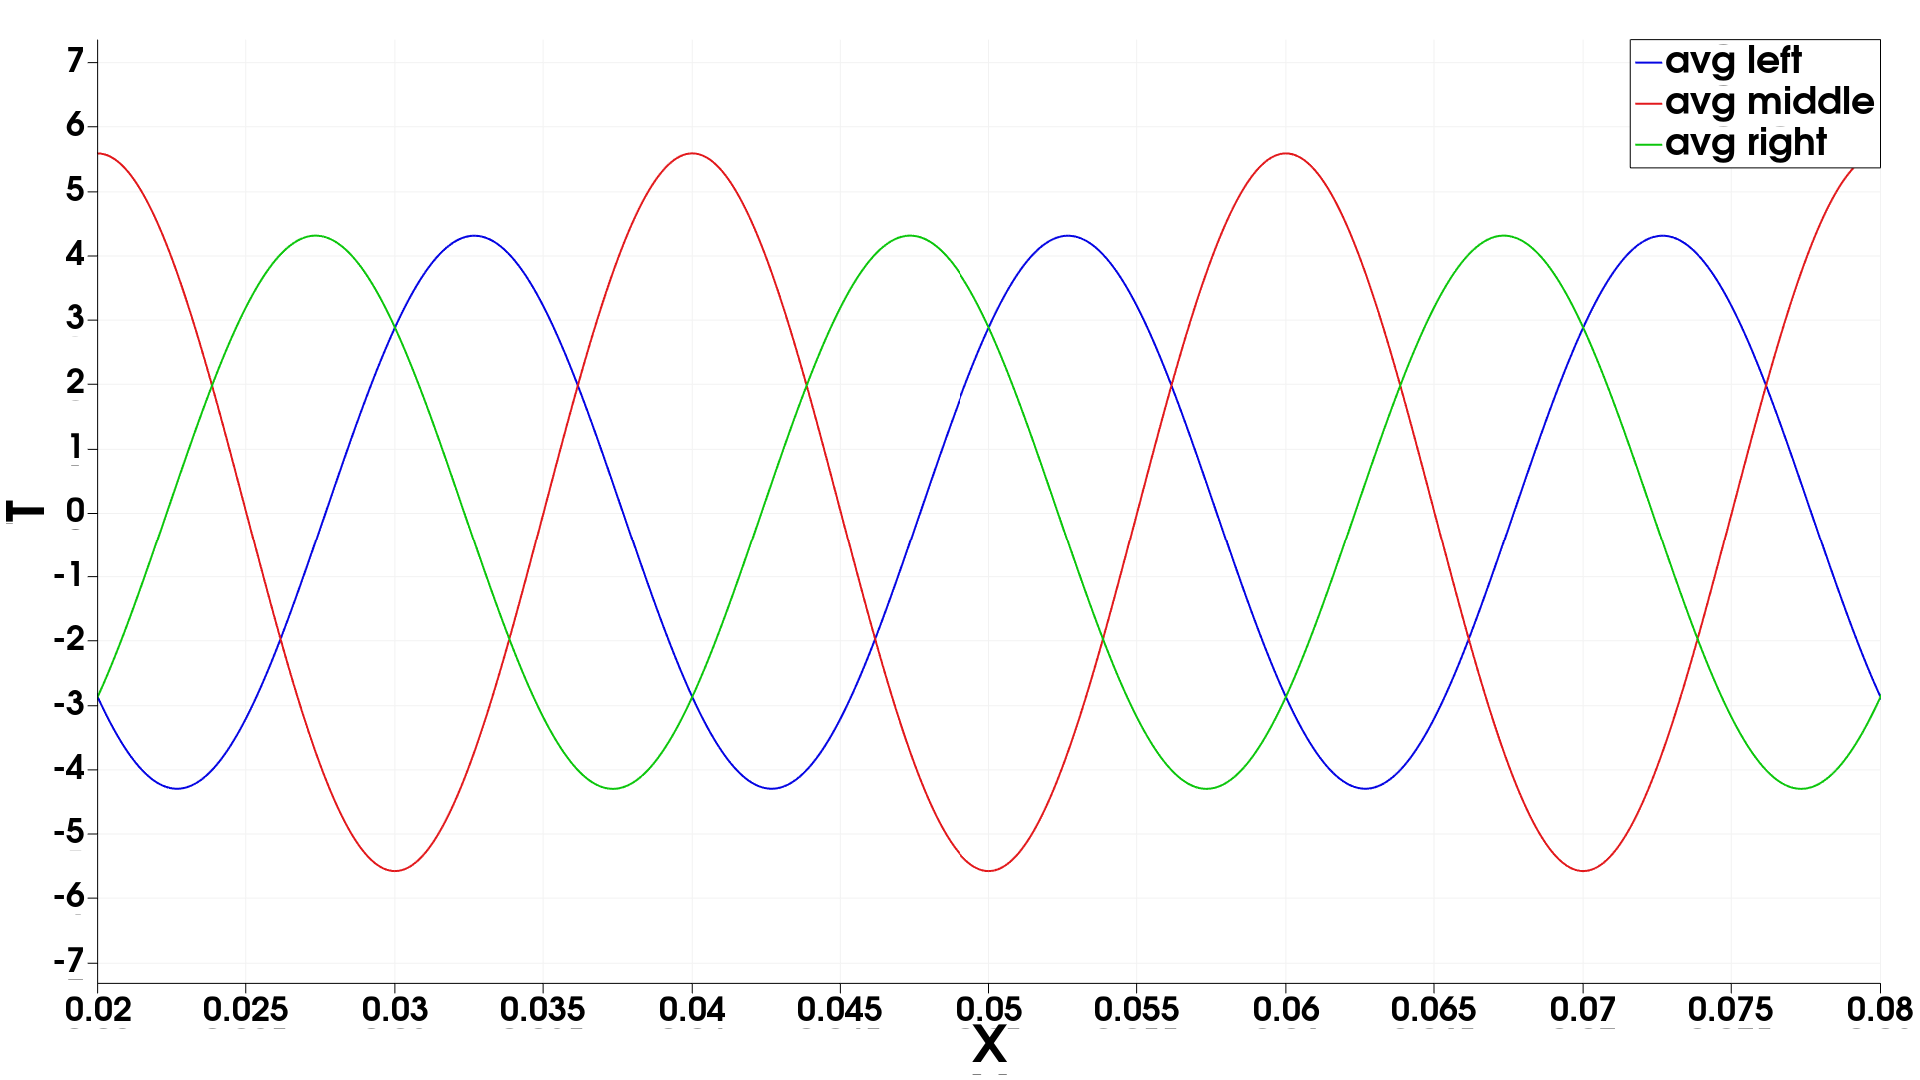
\includegraphics[width=0.8\textwidth]{img/B_phase_plot_linear_mu.png}
    \caption{Phase plot of $B$ for the linear model.}
    \label{fig:linear_model}
\end{figure}


\section{Non-linear Behaviour}


\begin{figure}[t]
    \centering
    \includegraphics[width=0.8\textwidth]{phaseplot_b_nonlinear.eps}
    \caption{Phase plot of $B$ for the non-linear model.}
    \label{fig:nonlinear_phaseplot}
\end{figure}



\begin{figure}[t]
    \centering
    \includegraphics[width=0.8\textwidth]{bnorm_t0.004.eps}
    \caption{Bnorm for the non-linear model.}
    \label{fig:nonlinear_bnorm}
\end{figure}


\begin{figure}[t]
    \centering
    \includegraphics[width=0.8\textwidth]{permeability_t0.004.eps}
    \caption{Permeability for the non-linear model.}
    \label{fig:nonlinear_permeability}
\end{figure}


\begin{figure}[t]
    \centering
    \includegraphics[width=0.8\textwidth]{permeability_nonlinear.eps}
    \caption{Permeability as a function of $||B||$.}
    \label{fig:nonlinear_permeability_bnorm}
\end{figure}

\section{Skin effect for higher harmonics}




